\documentclass[12pt, titlepage]{article}
\usepackage{tabularx}
\usepackage[left=2cm, right=2cm, top=2cm, bottom=2cm]{geometry}
\usepackage[utf8]{inputenc}
\usepackage{color}
\usepackage{graphicx}
\usepackage{amsmath}
\usepackage{tikz-timing}
\usepackage{setspace}
\usepackage{float}
\doublespacing

\newcommand{\pnote}[1]{{\langle \text{#1} \rangle}}

\title{
McMaster University\\
SFWRENG 4G06\\
\bigskip\bigskip\bigskip
{\bf Tip of My Shoe - SRS\\}
\bigskip\bigskip\bigskip\bigskip
\begin{table}[h!]
\begin{center}
\begin{tabular}{|p{5cm}|p{5cm}|p{5cm}|}
	\hline
	\bf Member Name & \bf Mac ID & \bf Student Number\\
	\hline
	\hline
	Chris Dibussolo & dibussoc & 400070368\\
	\hline
    Andrew Lucentini & lucenta & 001430150\\
    \hline
	Owen McNeil & mcneilo & 400065750 \\
	\hline
	Daniel Scime & scimed1 & 400069926\\
	\hline
    Ashley Williams & willia18 & 400081787\\
	\hline
      Lucas Zacharewicz & zacharel & 400054446\\
	\hline
\end{tabular}
\end{center}
\end{table}
\date{\today}
}

\usepackage{natbib}
\usepackage{graphicx}

\begin{document}

\maketitle
\tableofcontents
\newpage

% -----------------------------------------------------------------------------

\section{Overview}

\subsection{Purpose}
The purpose of this document is to present a functional and non-functional description for the software application titled \textbf{Tip of My Shoe}. The document shall elaborate on the overall description, functional requirements, and non-functional requirements of the software. This document is intended for developers, stakeholders, and users of the application

\subsection{Scope}

Tip of My Shoe will allow users to provide a picture of a shoe, in order to receive an identical/similar list of shoes provided via web-store link as to where the shoe can be purchased. The shoes will be sorted by highest matching. The project is intended (but not limited) to be administered as a smart-phone application. The project will incorporate numerous front-end and back-end technologies in-order to create a fully functioning user interface. Specific functionality is provided in the Functional Requirements section of this document.

\subsection{Stakeholders}

\subsubsection{The Client}
The clients are the members software team designing this project. It is not being created for an external client with external problems or goals. Any and all requirements come from the software team in this case.

\subsubsection{The Customers}
The customers will be any end user of the program. All requirements and functionalities are made with the end users in mind. Design will be conducted in a way such that the end application has a minimal and simplistic, yet concise interface. The experience should be easy and not frustrating for the user.

\subsection{Normal Operation/Use Case}
\begin{enumerate}
    \item User sees a shoe that they are interested in finding matches for.
    \item User takes a picture of shoe, preferably from the side profile of the shoe.
    \item User uploads picture to the program.
    \item After some small amount of wait time, the user will receive pictures and clickable links to similar shoes.
    \item User can either stay on the same page, click a link, or reset the program by uploading another picture.
    
\end{enumerate}

\subsection{Context Diagram}

\begin{figure}[!htbp]
  \centering
  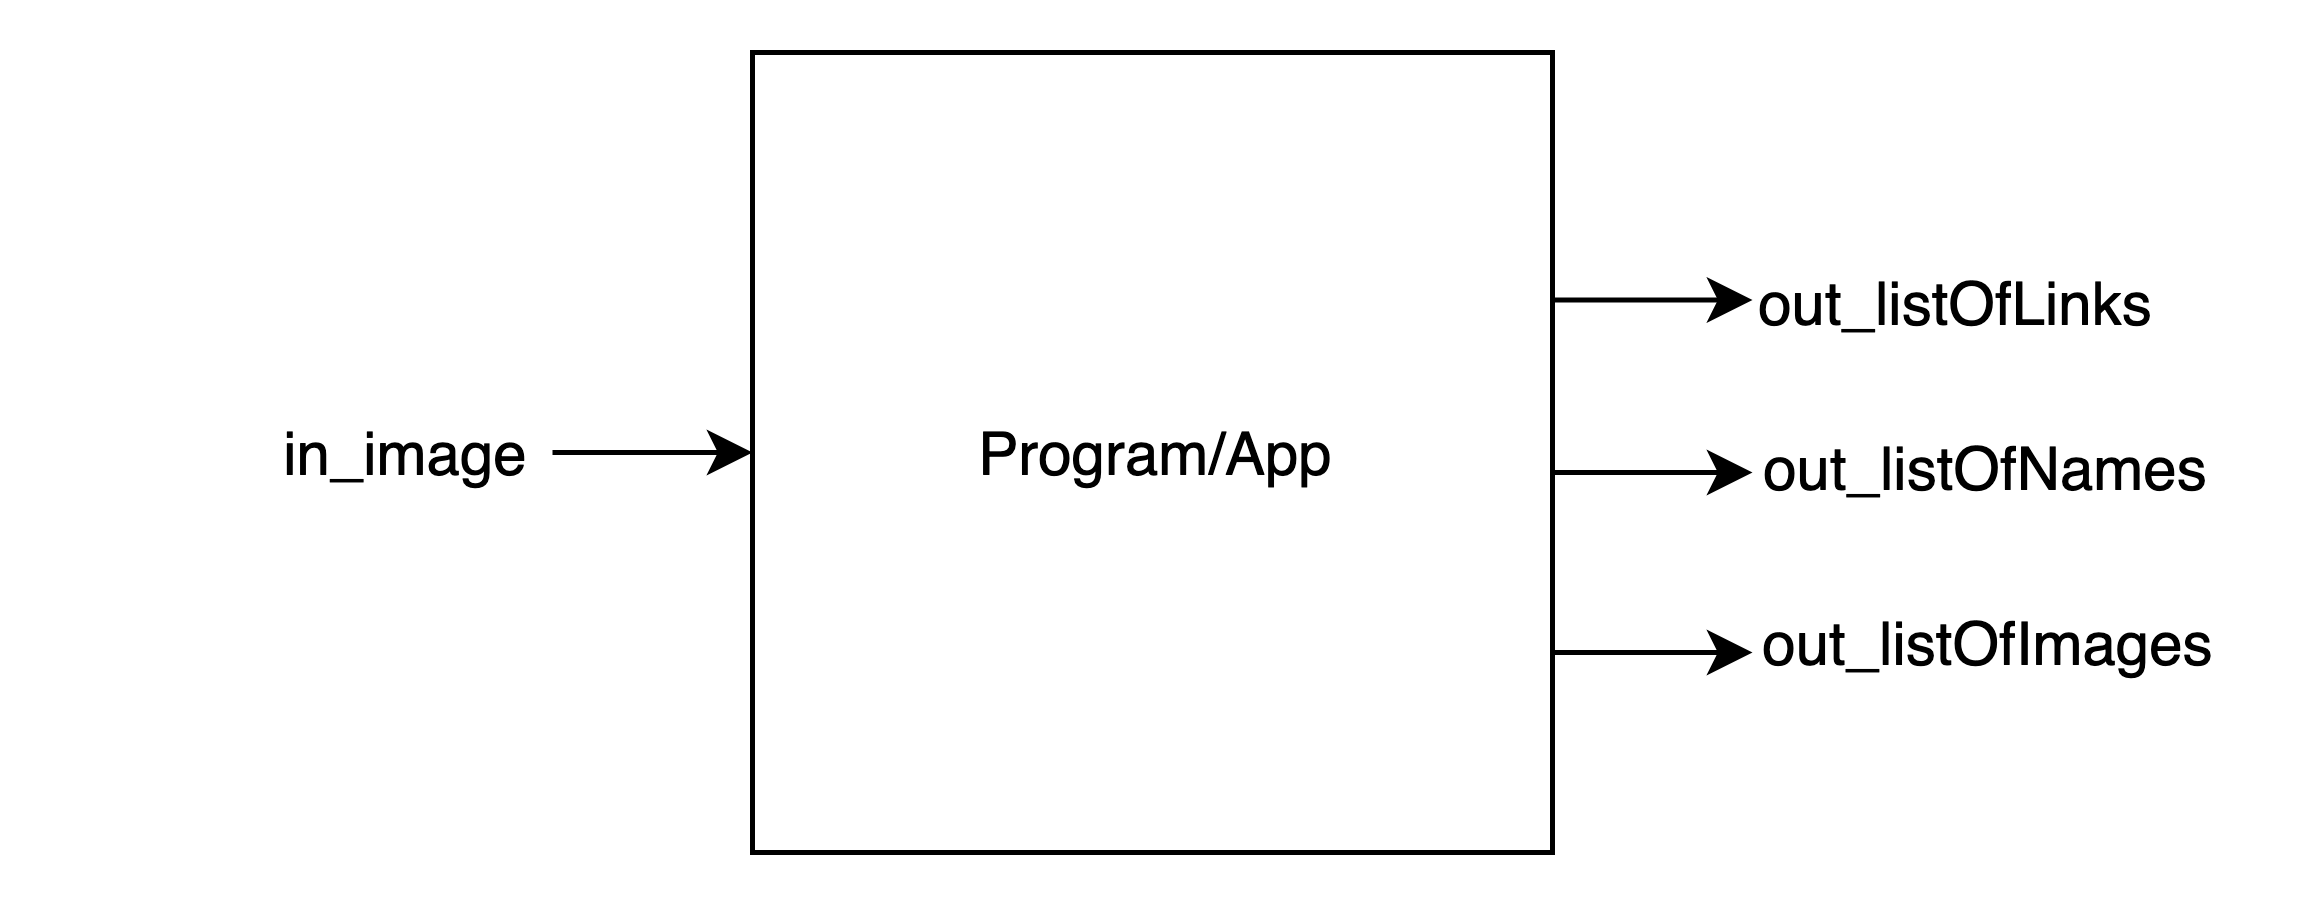
\includegraphics[width=0.8\textwidth]{images/Context-Diagram.png}
  \caption{Context Diagram}
\end{figure}

\newpage
\subsection{System Level Variables}

\subsubsection{Monitored Variables}

\begin{table}[!htbp]
\begin{center}
\begin{tabular}{|p{5cm}|p{10cm}|}
	\hline
	\bf Variable & \bf Description \\
	\hline
	in\_image & Input image taken from user. Compared to database of images in order to find similarities. \\
	\hline
\end{tabular}
\caption{Monitored Variables}
\end{center}
\end{table}

\subsubsection{Controlled Variables}

\begin{table}[!htbp]
\begin{center}
\begin{tabular}{|p{5cm}|p{10cm}|}
	\hline
	\bf Variable & \bf Description \\
	\hline
    out\_listOfNames & Output list of names of shoes. Each will have corresponding images and links. \\
	\hline
	out\_listOfLinks & Output list of links corresponding to different shoes. \\
	\hline
    out\_listOfImages & Output list of images. Found through backend algorithms with input image. \\
	\hline
\end{tabular}
\caption{Controlled Variables}
\end{center}
\end{table}

\subsubsection{Constants}

\begin{table}[!htbp]
\begin{center}
\begin{tabular}{|p{5cm}|p{10cm}|}
	\hline
	\bf Constant & \bf Description \\
	\hline
	Database Of Names & List of all currently acquired names of shoes. Stored internally for access when needed. \\
	\hline
	Database Of Links & List of all currently acquired links corresponding to different shoes. \\
	\hline
	Database Of Images & List of all currently acquired images of shoes. Used by comparing to input image. \\
	\hline
\end{tabular}
\caption{Constants}
\end{center}
\end{table}

% \subsubsection{Relevant Facts}

% \begin{itemize}
% \item
% \end{itemize}

\subsubsection{Relevant Assumptions}

The target user of this product is assumed to:
\begin{itemize}
\item Have general phone/computer knowledge. Specifically able to locate a picture file and upload it to the system.
\item Understand basic signifiers. One example would be highlighted links should be assumed clickable without specific instructions.
\end{itemize}

\section{Functional Requirements}


\subsection{Functional Requirements and Behaviour Overview}

\subsubsection{Overview of Product Behaviour}
\paragraph{} Tip Of My Shoe will provide users a list of shoes (via web-store links) that match a shoe that the user desires to purchase. The user will submit the design via a picture of a shoe. The software should match the patterns and overall design of the shoe to provide the user with results of retail products that would provide a similar look.


\subsubsection{Functional Decomposition}

\begin{figure}[H]
  \centering
  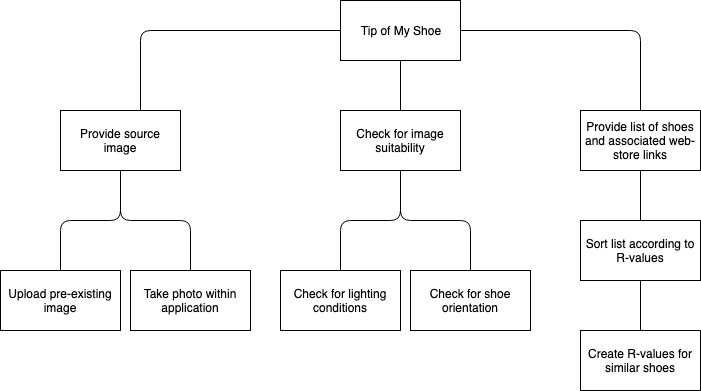
\includegraphics[width=0.8\textwidth]{images/Functional-Decomposition.png}
  \caption{Functional Decomposition Diagram}
\end{figure}


\subsubsection{Required Functions}
\begin{itemize}
    \item 
    \textbf{FR1:} The system will allow the user to upload an image or take a picture within the application. 
    
    \textbf{Rationale:} The user may already have an image of the shoe they are interested in, or may want to take their own photo without storing it on their device.
    
    \item 
    \textbf{FR2:} The system will only accept images of a specific form (e.g. suitable lighting conditions, shoe orientation) and will notify the user when an image is not usable. 
    
    \textbf{Rationale:} A clear photo of the shoe must be provided in order to identify it. Additionally, images provided by retailers are typically taken from specific views/orientations. Since identification will be based on these images, the source image should be in a similar form.
    
    \item 
    \textbf{FR3:} The system shall provide a list of shoes to the user that resemble some source image of a shoe. 
    
    \textbf{Rationale:} This is the main goal of the project, however, some liberties may be taken. For example, if it proves too difficult to provide multiple matches that resemble the shoe in the image to create a similar "look", we may opt to make the goal to find a retail seller of the exact shoe in the image should it be available. The subjective nature of matching the "look" of a shoe may prove much more difficult than definitively matching a set of parameters.
    
    \item 
    \textbf{FR4:} Provided shoes should have an associated "related value" (R-value). This R-value measures how similar the resulting shoe is to the searched shoe. 
    
    \textbf{Rationale:} This value will put a measure to the subjective concept of "how much does this shoe look like what I want?".
    
    \item 
    \textbf{FR5:} 
    
    \textbf{Rationale:} 
\end{itemize}

\section{Non-functional Requirements}

\subsection{Usability and Humanity Requirements}
This section is concerned with requirements that make the product usable and acceptable to the users. This is an important factor pertaining to our project.

\subsubsection{Ease of Use Requirements}
\begin{itemize}{}
    \item \textbf{Requirement:} The software should be usable by all potential customers within reason. The target age is 8+ years old.
    
    \textbf{Rationale:} Maximizing the domain of users will allow for large data collection, hence more accurate results.
    
    \item \textbf{Requirements:} The user should be able to easily operate the camera with minimal instructions.
    
    \textbf{Rationale:} The camera is the main means of searching for shoes based on an image taken by the user (a picture not taken from the internet or some secondary source). The camera should have on-screen instructions and automated aid for the user so minimal issues are experienced.
    
    \item \textbf{Requirements:} The interface should provide a simplistic sense of navigation through the program.
    
    \textbf{Rationale:} To promote repeated use, the user should not experience any issues in trying to figure out how to do what they want to do.
\end{itemize}

\subsubsection{Personalising and Internationalization Requirements}
\begin{itemize}
    \item\textbf{Requirements:} Users should eventually be usable to people of multiple nationalities, however, will predominantly focus on a western release, focusing on USA and Canada accessibility for anglophone users.
    
    \textbf{Rationale:} Given that the main challenge is making the software work, internationalization should be a task left for post. Initially, resources should be allocated to focusing on development for strictly English users in North America.
\end{itemize}

\subsubsection{Learning Requirements}
\begin{itemize}
    \item \textbf{Requirements:} The user should require minimal learning to understand how to use the software. On-screen instructions and intuitive interfacing should provide a seamless experience for the user.
    
    \textbf{Rationale:} Inherently, the use of the product is fairly simple, all the hard work is done by the software. All the user has to do is supply an image for their search. The process of supplying said image should therefore be made as easy as possible for the user so they do not have to learn anything complicated about how the software works.
\end{itemize}

\subsubsection{Understandability and Politeness Requirements}
\begin{itemize}
    \item \textbf{Requirements:} The overall usage and purpose of the software should be made easily apparent to the user. The user should not have to wonder what they are using the software for.
    
    \textbf{Rationale:} Given the niche nature of the software, it should be made very apparent to the user what exactly they are using it for.
\end{itemize}

\subsubsection{Accessibility Requirements}
\begin{itemize}
    \item \textbf{Requirements:} The software should be accessible by anyone with a smartphone or computer on a number of operating systems.
    
    \textbf{Rationale:} Primarily, the software should be available and provide solid performance on Windows 7-10 and MacOSX for PC users as well as Android and IOS for mobile users, given that these are the most likely ways for our target audience to be using the software. 
\end{itemize}

\subsection{Performance Requirements}
This section is concerned with requirements regarding the performance of the system.
\subsubsection{Speed and Latency Requirements}
\begin{itemize}
    \item \textbf{Requirement:} The software's search process should take no longer than 5 seconds to complete.
    
    \textbf{Rationale:} A search process longer than 10 seconds will make the user think the software is unreliable and they will be unlikely to use again. Similarly, if the user is waiting for 10 seconds for every image they search, they will be discouraged from using the software extensively.
\end{itemize}

\subsubsection{Safety-Critical Requirements}
\begin{itemize}
    \item \textbf{Requirement:} The software must not put excessive strain on the CPU so as to overheat the hardware.
    
    \textbf{Rationale:} We want to minize the risk of a hardware faiure. This can be accomplished by minimizing the strain on the CPU.
\end{itemize}

\subsubsection{Precision or Accuracy Requirements}
\begin{itemize} 
    \item 
    \textbf{Requirement:} The system must return shoes with R-values greater than 0.8.
    
    \textbf{Rationale:} The system must provide meaningful results.
    
    \item 
    \textbf{Requirement:} A list of similar shoes shall be provided to users if the system is unable to find an identical match.
    
    \textbf{Rationale:} In the case that a shoe cannot be found, we must provide the users with meaningful results.
    
    
    \item 
    \textbf{Requirement:} The similarity between the desired (user searched) and resulting shoe/shoes must be measurable by a defined scale through a combination of factors.
    
    \textbf{Rationale:} By measuring the "similarity" between desired and resulting shoe/shoes, we are able to identify the accuracy and efficiency of the system.
    
    
\end{itemize}


\subsubsection{Reliability and Availability Requirements}
\begin{itemize}
    \item \textbf{Requirement:} The software should maintain 99\% up-time.
    
    \textbf{Rationale:} This percentage means that for every 100 days only 24 hours of downtime should be expected. This time is left for maintenance and future patches of the software. Excessive down-time will make users unlikely to ever use the product given the niche nature of the product. Most people will assume it is too convenient to be true, and experiencing downtime will make them give up any expectation.
\end{itemize}

\subsubsection{Robustness or Fault-Tolerance Requirements}
\begin{itemize}
    \item \textbf{Requirement:} In the event of an error, particularly due to user input, the software should be able to handle the error without crashing and administer appropriate feedback to the user to ensure appropriate input is received.
    
    \textbf{Rationale:} A robust software should be able to handle undesired user input without a catastrophic system crash. To avoid recurring errors the system should provide the user with appropriate signifiers and feedback to ensure minimal errors occur. This also reinforces the desired seamless usability of the software.
    
    \item \textbf{Requirement:} In the event of a catastrophic failure (unhandled failure), the application should identify the failure upon re-opening.
    
    \textbf{Rationale:} A user who experience a program crash with no sense of aid from the system or instructions to proceed towards recovery is likely to not use the product again.
\end{itemize}

\subsubsection{Capacity Requirements}
\begin{itemize}
    \item \textbf{Requirement:} The system shall handle the processing of 10,000 simultaneous users.
    
    \textbf{Rationale:} Based on expected user growth, allowing the system to handle 10,000 simultaneous users will ensure that the system does not need functional modification for the years to come.
    
    \item \textbf{Requirement:} Server space will be required to support user accounts and store user data for the sake of machine learning and increasing the data set for the machine learning process.
    
    \textbf{Rationale:} Machine learning requires extensive data sets and along with web scraping it is likely that it will be necessary to store user data to make these data sets robust, making the search as accurate as possible.
\end{itemize}

\subsection{Security and Legal Requirements}
\subsubsection{Integrity Requirements}
\begin{itemize}
\item 
    \textbf{Requirement:} The system must ensure that all information will be stored on servers via encryption.
    
    \textbf{Rationale:} Should the software support user account data be secure to avoid loss of system credibility and endangering the user, especially if important information such as location is saved to the user account. Should the system be successful and a subscription fee be hypothetically in the future, the encryption of a user's financial information would also be critical.
\end{itemize}

\subsubsection{Privacy Requirements}
\begin{itemize}
\item 
    \textbf{Requirement:} The system must ensure that no privacy laws are broken.
    
    \textbf{Rationale:} Obvious reasons. We don't want no trouble.
\end{itemize}

\section{Undesired Scenario Handling}
The following sub sections pertain to scenarios in which the system may not behave correctly, and how corrective action will be taken in these situations.
\subsection{The System Cannot Extract Information from the Image}

There may be situations in which the picture provided to the system is inadequate for the system to extract information. The system will be able to identify this situation, and request that users provide a "better" image. The system will also provide the reason for error (i.e "This image is too dark").

\subsection{The System Cannot Find Close Matches}

If the system cannot find any close matches, it must the system must notify the user of this case. In addition, the system must provide shoes that have a lower R-Value than 0.8.

\subsection{Software Failure (General)}

If the system fails due to an unexpected software failure, the system must notify the user that the application has crashed once the user re-opens the application.


\section{Possible Changes and Noteable Risks}
\subsection{Requirements That Are Likely to Change}

\subsection{Requirements That Are Not Likely to Change}

\subsection{Risks}
\subsubsection{Excessive Schedule Pressure}
\paragraph{} Due to the nature of the project and the teams inexperience with machine learning software, maintaining a manageable schedule may prove daunting, due to the unpredictability of any said tasks time consumption.

\subsubsection{Management Malpractice}
The team must ensure that they stay organized on their management of time and resources while working on the project as falling behind make them unable to deliver.

\subsubsection{Low Quality}
Excessive focus on fancy features beyond the scope of the project will lead to the team being overwhelmed and producing low quality software. The team should avoid this risk by focusing on consistency and reliability, making sure the simple features work properly, instead of producing unneeded features that create more problems.


\subsection{Costs}

% \newpage
% \section{References}
% \bibliographystyle{plainnat}
% \bibliography{SRS}

\end{document}
